% $Header: /u/gcmpack/manual/s_phys_pkgs/text/exch2.tex,v 1.13 2004/03/17 19:49:22 afe Exp $
% $Name:  $

%%  * Introduction
%%    o what it does, citations (refs go into mitgcm_manual.bib, 
%%      preferably in alphabetic order)
%%    o Equations 
%%  * Key subroutines and parameters
%%  * Reference material (auto generated from Protex and structured comments)
%%    o automatically inserted at \section{Reference} 


\section{exch2: Extended Cubed Sphere \mbox{Topology}}
\label{sec:exch2}


\subsection{Introduction}

The \texttt{exch2} package extends the original cubed
sphere topology configuration to allow more flexible domain
decomposition and parallelization.  Cube faces (also called
subdomains) may be divided into any number of tiles that divide evenly
into the grid point dimensions of the subdomain.  Furthermore, the
individual tiles can run on separate processors in different
combinations, and whether exchanges between particular tiles occur
between different processors is determined at runtime.  This
flexibility provides for manual compile-time load balancing across a
relatively arbitrary number of processors. \\

The exchange parameters are declared in
\filelink{pkg/exch2/W2\_EXCH2\_TOPOLOGY.h}{pkg-exch2-W2_EXCH2_TOPOLOGY.h}
and assigned in
\filelink{pkg/exch2/w2\_e2setup.F}{pkg-exch2-w2_e2setup.F}. The
validity of the cube topology depends on the \file{SIZE.h} file as
detailed below.  The default files provided in the release configure a
cubed sphere topology of six tiles, one per subdomain, each with
32$\times$32 grid points, all running on a single processor.  Both
files are generated by Matlab scripts in
\file{utils/exch2/matlab-topology-generator}; see Section
\ref{sec:topogen} \sectiontitle{Generating Topology Files for exch2}
for details on creating alternate topologies.  Pregenerated examples
of these files with alternate topologies are provided under
\file{utils/exch2/code-mods} along with the appropriate \file{SIZE.h}
file for single-processor execution.

\subsection{Invoking exch2}

To use exch2 with the cubed sphere, the following conditions must be
met: \\

$\bullet$ The exch2 package is included when \file{genmake2} is run.
  The easiest way to do this is to add the line \code{exch2} to the
  \file{profile.conf} file -- see Section
  \ref{sect:buildingCode} \sectiontitle{Building the code} for general
  details. \\

$\bullet$ An example of \file{W2\_EXCH2\_TOPOLOGY.h} and
  \file{w2\_e2setup.F} must reside in a directory containing code
  linked when \file{genmake2} runs.  The safest place to put these
  is the directory indicated in the \code{-mods=DIR} command line
  modifier (typically \file{../code}), or the build directory.  The
  default versions of these files reside in \file{pkg/exch2} and are
  linked automatically if no other versions exist elsewhere in the
  link path, but they should be left untouched to avoid breaking
  configurations other than the one you intend to modify.\\

$\bullet$ Files containing grid parameters, named
  \file{tile00$n$.mitgrid} where $n$=\code{(1:6)} (one per subdomain),
  must be in the working directory when the MITgcm executable is run.
  These files are provided in the example experiments for cubed sphere
  configurations with 32$\times$32 cube sides and are non-trivial to
  generate -- please contact MITgcm support if you want to generate
  files for other configurations. \\

$\bullet$ As always when compiling MITgcm, the file \file{SIZE.h} must
  be placed where \file{genmake2} will find it.  In particular for
  exch2, the domain decomposition specified in \file{SIZE.h} must
  correspond with the particular configuration's topology specified in
  \file{W2\_EXCH2\_TOPOLOGY.h} and \file{w2\_e2setup.F}.  Domain
  decomposition issues particular to exch2 are addressed in Section
  \ref{sec:topogen} \sectiontitle{Generating Topology Files for exch2}
  and \ref{sec:exch2mpi} \sectiontitle{exch2, SIZE.h, and MPI}; a more
  general background on the subject relevant to MITgcm is presented in
  Section \ref{sect:specifying_a_decomposition}
  \sectiontitle{Specifying a decomposition}.\\

As of the time of writing the following examples use exch2 and may be
used for guidance:

\begin{verbatim}
verification/adjust_nlfs.cs-32x32x1
verification/adjustment.cs-32x32x1 
verification/aim.5l_cs
verification/global_ocean.cs32x15
verification/hs94.cs-32x32x5
\end{verbatim}




\subsection{Generating Topology Files for exch2}
\label{sec:topogen}

Alternate cubed sphere topologies may be created using the Matlab
scripts in \file{utils/exch2/matlab-topology-generator}. Running the
m-file
\filelink{driver.m}{utils-exch2-matlab-topology-generator_driver.m}
from the Matlab prompt (there are no parameters to pass) generates
exch2 topology files \file{W2\_EXCH2\_TOPOLOGY.h} and
\file{w2\_e2setup.F} in the working directory and displays a figure of
the topology via Matlab.  The other m-files in the directory are
subroutines of \file{driver.m} and should not be run ``bare'' except
for development purposes. \\

The parameters that determine the dimensions and topology of the
generated configuration are \code{nr}, \code{nb}, \code{ng},
\code{tnx} and \code{tny}, and all are assigned early in the script. \\

The first three determine the size of the subdomains and
hence the size of the overall domain.  Each one determines the number
of grid points, and therefore the resolution, along the subdomain
sides in a ``great circle'' around an axis of the cube.  At the time
of this writing MITgcm requires these three parameters to be equal,
but they provide for future releases  to accomodate different
resolutions around the axes to allow (for example) greater resolution
around the equator.\\

The parameters \code{tnx} and \code{tny} determine the dimensions of
the tiles into which the subdomains are decomposed, and must evenly
divide the integer assigned to \code{nr}, \code{nb} and \code{ng}.
The result is a rectangular tiling of the subdomain.  Figure
\ref{fig:24tile} shows one possible topology for a twentyfour-tile
cube, and figure \ref{fig:12tile} shows one for twelve tiles. \\

\begin{figure}
\begin{center}
 \resizebox{4in}{!}{
  \includegraphics{part6/s24t_16x16.ps}
 }
\end{center} 

\caption{Plot of a cubed sphere topology with a 32$\times$192 domain
divided into six 32$\times$32 subdomains, each of which is divided into four tiles 
(\code{tnx=16, tny=16}) for a total of twentyfour tiles.
} \label{fig:24tile}
\end{figure}

\begin{figure}
\begin{center}
 \resizebox{4in}{!}{
  \includegraphics{part6/s12t_16x32.ps}
 }
\end{center} 
\caption{Plot of a cubed sphere topology with a 32$\times$192 domain
divided into six 32$\times$32 subdomains of two tiles each
 (\code{tnx=16, tny=32}).
} \label{fig:12tile}
\end{figure}

\begin{figure}
\begin{center}
 \resizebox{4in}{!}{
  \includegraphics{part6/s6t_32x32.ps}
 }
\end{center} 
\caption{Plot of a cubed sphere topology with a 32$\times$192 domain
divided into six 32$\times$32 subdomains with one tile each
(\code{tnx=32, tny=32}).  This is the default configuration.
  }
\label{fig:6tile}
\end{figure}


Tiles can be selected from the topology to be omitted from being
allocated memory and processors.  This tuning is useful in ocean
modeling for omitting tiles that fall entirely on land.  The tiles
omitted are specified in the file
\filelink{blanklist.txt}{utils-exch2-matlab-topology-generator_blanklist.txt}
by their tile number in the topology, separated by a newline. \\




\subsection{exch2, SIZE.h, and multiprocessing}
\label{sec:exch2mpi}

Once the topology configuration files are created, the Fortran
\code{PARAMETER}s in \file{SIZE.h} must be configured to match.
Section \ref{sect:specifying_a_decomposition} \sectiontitle{Specifying
a decomposition} provides a general description of domain
decomposition within MITgcm and its relation to \file{SIZE.h}. The
current section specifies certain constraints the exch2 package
imposes as well as describes how to enable parallel execution with
MPI. \\

As in the general case, the parameters \varlink{sNx}{sNx} and
\varlink{sNy}{sNy} define the size of the individual tiles, and so
must be assigned the same respective values as \code{tnx} and
\code{tny} in \file{driver.m}.\\

The halo width parameters \varlink{OLx}{OLx} and \varlink{OLy}{OLy}
have no special bearing on exch2 and may be assigned as in the general
case. The same holds for \varlink{Nr}{Nr}, the number of vertical 
levels in the model.\\

The parameters \varlink{nSx}{nSx}, \varlink{nSy}{nSy},
\varlink{nPx}{nPx}, and \varlink{nPy}{nPy} relate to the number of
tiles and how they are distributed on processors.  When using exch2,
the tiles are stored in single dimension, and so
\code{\varlink{nSy}{nSy}=1} in all cases.  Since the tiles as
configured by exch2 cannot be split up accross processors without
regenerating the topology, \code{\varlink{nPy}{nPy}=1} as well. \\

The number of tiles MITgcm allocates and how they are distributed
between processors depends on \varlink{nPx}{nPx} and
\varlink{nSx}{nSx}.  \varlink{nSx}{nSx} is the number of tiles per
processor and \varlink{nPx}{nPx} the number of processors.  The total
number of tiles in the topology minus those listed in
\file{blanklist.txt} must equal \code{nSx*nPx}. \\

The following is an example of \file{SIZE.h} for the twelve-tile
configuration illustrated in figure \ref{fig:12tile} running on 
one processor: \\

\begin{verbatim}
      PARAMETER (
     &           sNx =  16,
     &           sNy =  32,
     &           OLx =   2,
     &           OLy =   2,
     &           nSx =  12,
     &           nSy =   1,
     &           nPx =   1,
     &           nPy =   1,
     &           Nx  = sNx*nSx*nPx,
     &           Ny  = sNy*nSy*nPy,
     &           Nr  =   5)
\end{verbatim}

The following is an example for the twentyfour-tile topology in figure
\ref{fig:24tile} running on six processors:

\begin{verbatim}
      PARAMETER (
     &           sNx =  16,
     &           sNy =  16,
     &           OLx =   2,
     &           OLy =   2,
     &           nSx =   4,
     &           nSy =   1,
     &           nPx =   6,
     &           nPy =   1,
     &           Nx  = sNx*nSx*nPx,
     &           Ny  = sNy*nSy*nPy,
     &           Nr  =   5)
\end{verbatim}





\subsection{Key Variables}

The descriptions of the variables are divided up into scalars,
one-dimensional arrays indexed to the tile number, and two and three
dimensional arrays indexed to tile number and neighboring tile.  This
division reflects the functionality of these variables: The
scalars are common to every part of the topology, the tile-indexed
arrays to individual tiles, and the arrays indexed by tile and
neighbor to relationships between tiles and their neighbors. \\

\subsubsection{Scalars}

The number of tiles in a particular topology is set with the parameter
\code{NTILES}, and the maximum number of neighbors of any tiles by
\code{MAX\_NEIGHBOURS}.  These parameters are used for defining the
size of the various one and two dimensional arrays that store tile
parameters indexed to the tile number and are assigned in the files
generated by \file{driver.m}.\\

The scalar parameters \varlink{exch2\_domain\_nxt}{exch2_domain_nxt}
and \varlink{exch2\_domain\_nyt}{exch2_domain_nyt} express the number
of tiles in the $x$ and $y$ global indices.  For example, the default
setup of six tiles (Fig. \ref{fig:6tile}) has \code{exch2\_domain\_nxt=6} and
\code{exch2\_domain\_nyt=1}.  A topology of twenty-four square tiles,
four per subdomain (as in figure \ref{fig:24tile}), will have
\code{exch2\_domain\_nxt=12} and \code{exch2\_domain\_nyt=2}.  Note
that these parameters express the tile layout to allow global data
files that are tile-layout-neutral and have no bearing on the internal
storage of the arrays.  The tiles are internally stored in a range
from \code{(1:\varlink{bi}{bi})} the $x$ axis, and $y$ axis variable
\varlink{bj}{bj} is generally ignored within the package. \\

\subsubsection{Arrays Indexed to Tile Number}

The following arrays are of length \code{NTILES}, are indexed to the
tile number, and the indices are omitted in their descriptions. \\

The arrays \varlink{exch2\_tnx}{exch2_tnx} and
\varlink{exch2\_tny}{exch2_tny} express the $x$ and $y$ dimensions of
each tile.  At present for each tile \texttt{exch2\_tnx=sNx} and
\texttt{exch2\_tny=sNy}, as assigned in \file{SIZE.h} and described in
section \ref{sec:exch2mpi} \sectiontitle{exch2, SIZE.h, and
multiprocessing}.  Future releases of MITgcm are to allow varying tile
sizes. \\

The location of the tiles' Cartesian origin within a subdomain are
determined by the arrays \varlink{exch2\_tbasex}{exch2_tbasex} and
\varlink{exch2\_tbasey}{exch2_tbasey}.  These variables are used to
relate the location of the edges of different tiles to each other.  As
an example, in the default six-tile topology (Fig. \ref{fig:6tile})
each index in these arrays is set to \code{0} since a tile occupies
its entire subdomain.  The twentyfour-tile case discussed above will
have values of \code{0} or \code{16}, depending on the quadrant the
tile falls within the subdomain.  The elements of the arrays
\varlink{exch2\_txglobalo}{exch2_txglobalo} and
\varlink{exch2\_txglobalo}{exch2_txglobalo} are similar to
\varlink{exch2\_tbasex}{exch2_tbasex} and
\varlink{exch2\_tbasey}{exch2_tbasey}, but locate the tiles within the
global address space, similar to that used by global files. \\

The array \varlink{exch2\_myFace}{exch2_myFace} contains the number of
the subdomain of each tile, in a range \code{(1:6)} in the case of the
standard cube topology and indicated by \textbf{\textsf{f}}$n$ in
figures \ref{fig:12tile} and
\ref{fig:24tile}. \varlink{exch2\_nNeighbours}{exch2_nNeighbours}
contains a count of how many neighboring tiles each tile has, and is
used for setting bounds for looping over neighboring tiles.
\varlink{exch2\_tProc}{exch2_tProc} holds the process rank of each
tile, and is used in interprocess communication.  \\


The arrays \varlink{exch2\_isWedge}{exch2_isWedge},
\varlink{exch2\_isEedge}{exch2_isEedge},
\varlink{exch2\_isSedge}{exch2_isSedge}, and
\varlink{exch2\_isNedge}{exch2_isNedge} are set to \code{1} if the
indexed tile lies on the edge of a subdomain, \code{0} if not.  The
values are used within the topology generator to determine the
orientation of neighboring tiles, and to indicate whether a tile lies
on the corner of a subdomain.  The latter case requires special
exchange and numerical handling for the singularities at the eight
corners of the cube. \\


\subsubsection{Arrays Indexed to Tile Number and Neighbor}

The following arrays are all of size
\code{MAX\_NEIGHBOURS}$\times$\code{NTILES} and describe the
orientations between the the tiles. \\

The array \code{exch2\_neighbourId(a,T)} holds the tile number
\code{Tn} for each of the tile number \code{T}'s neighboring tiles
\code{a}.  The neighbor tiles are indexed \code{(1:MAX\_NEIGHBOURS)}
in the order right to left on the north then south edges, and then top
to bottom on the east and west edges.  Maybe throw in a fig here, eh?
\\

\sloppy
The \code{exch2\_opposingSend\_record(a,T)} array holds the index
\code{b} in \texttt{exch2\_neighbourId(b,Tn)} that holds the tile
number \code{T}.  In other words,
\begin{verbatim}
   exch2_neighbourId( exch2_opposingSend_record(a,T),
                      exch2_neighbourId(a,T) ) = T
\end{verbatim}
This provides a back-reference from the neighbor tiles. \\

The arrays \varlink{exch2\_pi}{exch2_pi} and
\varlink{exch2\_pj}{exch2_pj} specify the transformations of variables
in exchanges between the neighboring tiles.  These transformations are
necessary in exchanges between subdomains because a physical vector
component in one direction may map to one in a different direction in
an adjacent subdomain, and may be have its indexing reversed. This
swapping arises from the ``folding'' of two-dimensional arrays into a
three-dimensional cube.

The dimensions of \code{exch2\_pi(t,N,T)} and \code{exch2\_pj(t,N,T)}
are the neighbor ID \code{N} and the tile number \code{T} as explained
above, plus a vector of length 2 containing transformation factors
\code{t}.  The first element of the transformation vector indicates
the factor \code{t} by which variables representing the same
\emph{physical} vector component of a tile \code{T} will be multiplied
in exchanges with neighbor \code{N}, and the second element indicates
the transform to the physical vector in the other direction.  To
clarify (hopefully), \code{exch2\_pi(1,N,T)} holds the transform of
the $i$ component of a vector variable in tile \code{T} to the $i$
component of tile \code{T}'s neighbor \code{N}, and
\code{exch2\_pi(2,N,T)} holds the transform of \code{T}'s $i$
components to the neighbor \code{N}'s $j$ component. \\
 
Under the current cube topology, one of the two elements of
\code{exch2\_pi} or \code{exch2\_pj} for a given tile \code{T} and
neighbor \code{N} will be \code{0}, reflecting the fact that the two
vector components are orthogonal.  The other element will be \code{1}
or \code{-1}, depending on whether the components are indexed in the
same or opposite directions.  For example, the transform vector of the
arrays for all tile neighbors on the same subdomain will be
\code{(1,0)}, since all tiles on the same subdomain are oriented
identically.  A vector direction that corresponds to the orthogonal
dimension with the same index direction in a particular tile-neighbor
orientation will have \code{(0,1)}, whereas those in the opposite
index direction will have \code{(0,-1)}. \\


\varlink{exch2\_oi}{exch2_oi},
\varlink{exch2\_oj}{exch2_oj}, \varlink{exch2\_oi\_f}{exch2_oi_f}, and
\varlink{exch2\_oj\_f}{exch2_oj_f}




This needs some diagrams. \\


{\footnotesize
\begin{verbatim}
C      exch2_pi          :: X index row of target to source permutation 
C                        :: matrix for each neighbour entry.            
C      exch2_pj          :: Y index row of target to source permutation 
C                        :: matrix for each neighbour entry.            
C      exch2_oi          :: X index element of target to source 
C                        :: offset vector for cell-centered quantities  
C                        :: of each neighbor entry.                     
C      exch2_oj          :: Y index element of target to source 
C                        :: offset vector for cell-centered quantities  
C                        :: of each neighbor entry.                     
C      exch2_oi_f        :: X index element of target to source 
C                        :: offset vector for face quantities           
C                        :: of each neighbor entry.                     
C      exch2_oj_f        :: Y index element of target to source 
C                        :: offset vector for face quantities           
C                        :: of each neighbor entry.                     
\end{verbatim}
}



\subsection{Key Routines}



\subsection{References}
